\documentclass[conference]{IEEEtran}
\IEEEoverridecommandlockouts

\usepackage{cite}
\usepackage{amsmath,amssymb,amsfonts}
\usepackage{graphicx}
\usepackage{textcomp}
\usepackage{xcolor}
\usepackage{booktabs}
\usepackage{url}

\graphicspath{{figures/}{report_finalization/figures/}}

\def\BibTeX{{\rm B\kern-.05em{\sc i\kern-.025em b}\kern-.08em
    T\kern-.1667em\lower.7ex\hbox{E}\kern-.125emX}}

\begin{document}

\title{Efficient UAV Small-Object Detection with Binary Scout-Guided Selective Tiling}

\author{
\IEEEauthorblockN{Student 1, Student 2, Student 3, Student 4}
\IEEEauthorblockA{Oslo Metropolitan University\\
ACIT4630 Advanced Machine Learning and Deep Learning}
}

\maketitle

\begin{abstract}
Write this last. It should state the problem, method, dataset, key result, and honest conclusion in one compact paragraph. Safe result wording: exhaustive tiled YOLO improved small-object recall from 0.084 to 0.355 on the 100-image validation benchmark, while oracle tile selection showed that a small tile subset can recover most of this gain. The implemented binary/XNOR scout recovered part of the tiling benefit, but did not meet the strict K18 recall/latency target, so the final result is partial validation rather than a solved edge-deployment system.
\end{abstract}

\begin{IEEEkeywords}
small object detection, UAV imagery, YOLO, selective tiling, binary neural networks, XNOR-popcount, edge inference
\end{IEEEkeywords}

\section{Introduction}
Small objects in UAV imagery are difficult for standard object detectors because resizing a full high-resolution frame to a fixed detector input can shrink objects to only a few pixels. Exhaustive tiled inference preserves more detail by running the detector on overlapping crops, but it multiplies detector calls and is difficult to justify for drone-like compute budgets.

This project evaluates a selective tiling alternative. A cheap scout model first scores candidate tiles, then YOLO runs only on selected original-resolution crops, and detections are merged back into the image coordinate system. The project is motivated by the idea that a binary/XNOR-popcount scout could select useful tiles at low cost while leaving accurate object detection to YOLO.

The contribution is a measured ML systems pipeline, not a new detector architecture. The report should emphasize three questions: how much small-object recall tiling adds, how much of that gain is theoretically recoverable with few tiles, and how close the learned binary/XNOR scout gets to that oracle opportunity under realistic timing.

\section{Background and Related Work}
VisDrone provides UAV detection data with many small, dense objects \cite{zhu2020visdrone}. YOLO-style detectors provide fast one-stage inference and are a practical baseline for deployment-oriented object detection \cite{ultralyticsYoloDocs}. SAHI-style slicing improves small-object detection by preserving local resolution, but increases the number of detector inputs \cite{akyon2022sahi}.

Binary neural networks and XNOR-popcount inference reduce arithmetic cost by replacing high-precision multiply-add operations with bitwise operations \cite{rastegari2016xnor}. In this project, the binary model is not a detector replacement. It is a scout/router: it estimates which tiles are worth sending to YOLO.

\section{Proposed Solution}
The implemented pipeline is:
\[
\text{image} \rightarrow \text{binary scout scores} \rightarrow \text{top-}K\text{ tiles}
\rightarrow \text{YOLO on selected crops} \rightarrow \text{merged detections}.
\]
Images are evaluated on a fixed 49-tile grid over a 640 evaluation canvas. Tiled detector runs use original-resolution crops projected from the selected 640-grid tiles. This preserves the high-resolution tiling claim while keeping one consistent evaluation coordinate system.

The final binary/XNOR route uses a 320-input STE heatmap scout exported to a native CPU XNOR-popcount path. The scout produces tile scores; tile-NMS selects the highest-value tiles; YOLOv8n runs on selected crops on the GPU; detections are merged with NMS. A learned GPU heatmap scout is included as a ranking/speed reference on the RTX 4090, not as the deployment target.

\begin{figure}[t]
\centering
\fbox{\begin{minipage}{0.92\linewidth}
\centering
Image $\rightarrow$ 49 candidate tiles $\rightarrow$ binary/XNOR scout heatmap $\rightarrow$ top-$K$ tile crops $\rightarrow$ YOLO detections $\rightarrow$ merged output.
\end{minipage}}
\caption{Scout-guided selective tiling. The scout only routes tiles; YOLO remains the final detector.}
\label{fig:pipeline}
\end{figure}

\section{Implementation}
The repository is organized around explicit data contracts rather than a large framework. The tile contract is fixed at 160-pixel tiles, stride 80, and 49 candidate tiles on the 640 evaluation canvas. \texttt{src/kernel.c} implements the native XNOR-popcount primitive, \texttt{src/xnor\_heatmap\_scout.py} connects the trained STE scout to native binary inference, and \texttt{scripts/run\_yolo\_tiles.py} runs the end-to-end detector routing benchmark.

The implementation keeps detector behavior fixed during the final benchmark: the YOLO weights, detector loss, tile grid, crop geometry, merge logic, NMS settings, and validation subset are unchanged across compared methods. This isolates the routing question. The custom detector loss discussed in the presentation is left as future work because adding detector fine-tuning would change the experimental question.

\section{Experimental Setup}
The final benchmark uses the first 100 official VisDrone validation images, COCO-pretrained \texttt{yolov8n.pt}, a Windows desktop with an RTX 4090 FE, CUDA PyTorch, original-resolution crops for tiled methods, and one warmup image. Results are class-agnostic recall and small-object recall on the 640 evaluation canvas. These are pipeline validation metrics, not official VisDrone mAP.

The compared methods are full-image YOLO, exhaustive tiled YOLO over all 49 tiles, oracle greedy tile selection, learned GPU heatmap scouts, objectness-trained XNOR scouts, and oracle-rank-trained XNOR scouts. The oracle is not deployable because it uses ground truth; it is included to measure the best possible tile-selection opportunity.

\section{Results}
Table~\ref{tab:final_detector} gives the main detector benchmark. Full-image YOLO is fastest but has low small-object recall. Exhaustive tiled YOLO has the highest measured recall but is much slower. Oracle selection shows that much of the tiling benefit is recoverable with far fewer tiles.

\begin{table}[t]
\centering
\caption{Final detector benchmark on 100 VisDrone validation images. Tiled methods use original-resolution crops.}
\label{tab:final_detector}
\begin{tabular}{lrrrrr}
\toprule
Method & $K$ & Recall & Small recall & Tiles & Mean ms \\
\midrule
Full YOLO & -- & 0.129 & 0.084 & 0 & 13.7 \\
Exhaustive tiled YOLO & 49 & 0.399 & 0.355 & 49 & 107.2 \\
Oracle greedy & 12 & 0.363 & 0.329 & 12 & 32.9 \\
Oracle greedy & 18 & 0.384 & 0.345 & 18 & 44.0 \\
Learned GPU objectness & 20 & 0.357 & 0.317 & 20 & 54.6 \\
Objectness XNOR & 18 & 0.343 & 0.306 & 18 & 64.0 \\
Oracle-rank XNOR & 18 & 0.344 & 0.309 & 18 & 63.8 \\
Oracle-rank XNOR & 24 & 0.361 & 0.320 & 24 & 75.8 \\
\bottomrule
\end{tabular}
\end{table}

\begin{figure}[t]
\centering
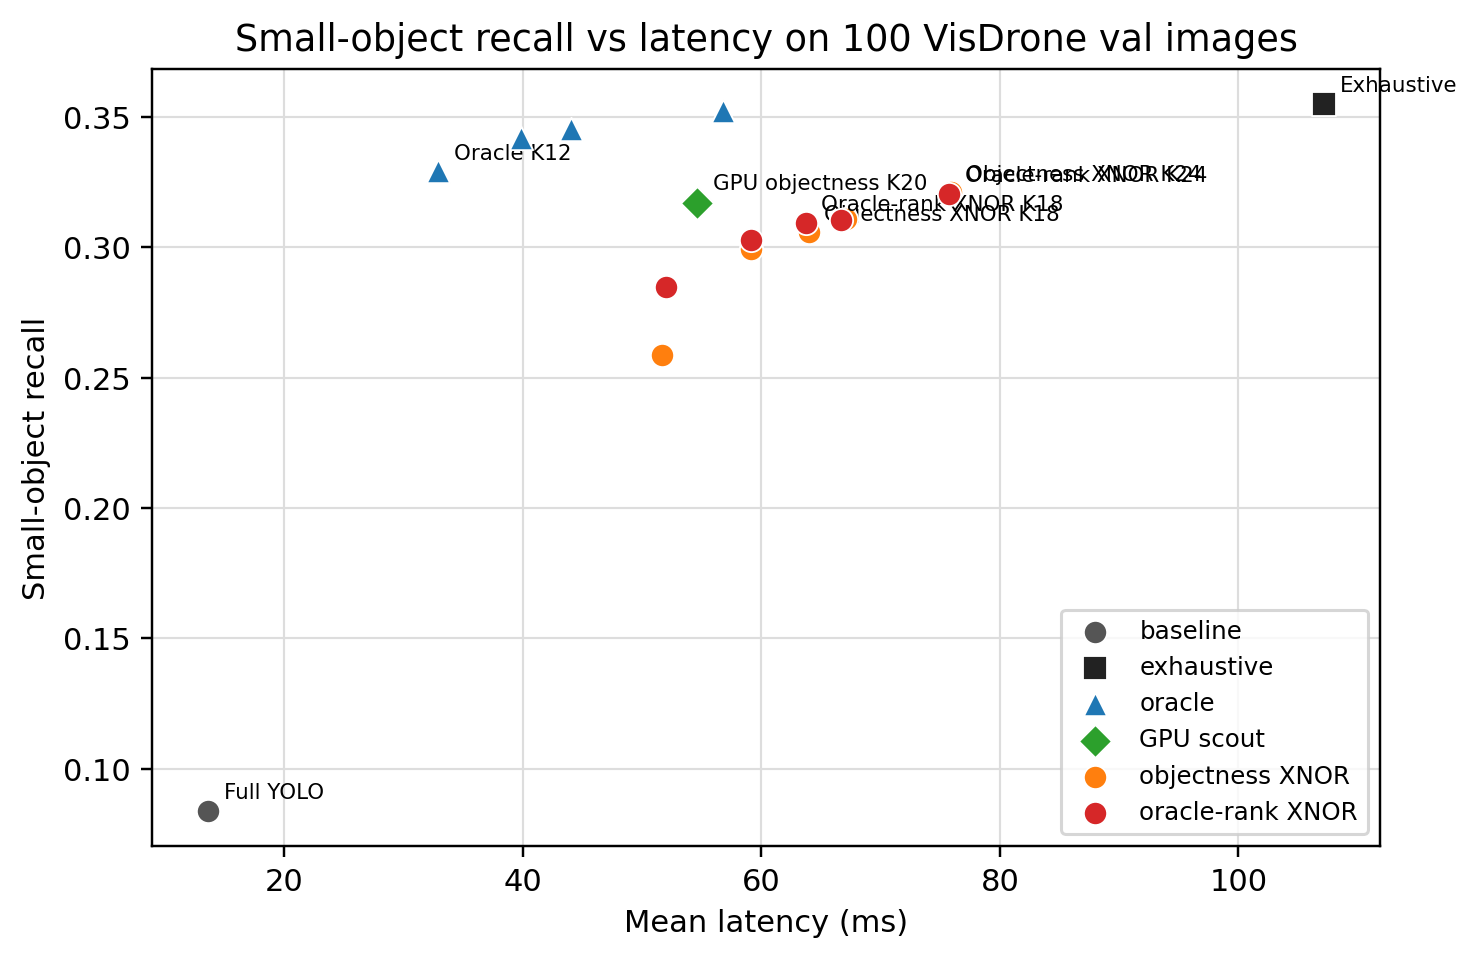
\includegraphics[width=\linewidth]{small_recall_vs_latency.png}
\caption{Small-object recall versus mean latency. Oracle routing shows the available opportunity; the XNOR scout partially closes the gap but misses the strict K18 target.}
\label{fig:small_recall_latency}
\end{figure}

Table~\ref{tab:xnor_sweep} compares the two final native XNOR scout training targets. Oracle-rank supervision improves low-K scout-only ranking and improves detector-level K12 recall, but the detector-level K18 result remains below the target of 0.355 overall recall, 0.318 small recall, and at most 60.1 ms latency.

\begin{table}[t]
\centering
\caption{Native XNOR detector K-sweep. Oracle-rank supervision helps low-K routing but does not reach the strict K18 success target.}
\label{tab:xnor_sweep}
\begin{tabular}{lrrrr}
\toprule
Route & $K$ & Recall & Small recall & Mean ms \\
\midrule
Objectness XNOR & 12 & 0.299 & 0.259 & 51.7 \\
Oracle-rank XNOR & 12 & 0.316 & 0.285 & 52.1 \\
Objectness XNOR & 16 & 0.336 & 0.299 & 59.1 \\
Oracle-rank XNOR & 16 & 0.338 & 0.303 & 59.2 \\
Objectness XNOR & 18 & 0.343 & 0.306 & 64.0 \\
Oracle-rank XNOR & 18 & 0.344 & 0.309 & 63.8 \\
Objectness XNOR & 24 & 0.363 & 0.321 & 75.9 \\
Oracle-rank XNOR & 24 & 0.361 & 0.320 & 75.8 \\
\bottomrule
\end{tabular}
\end{table}

\begin{figure}[t]
\centering
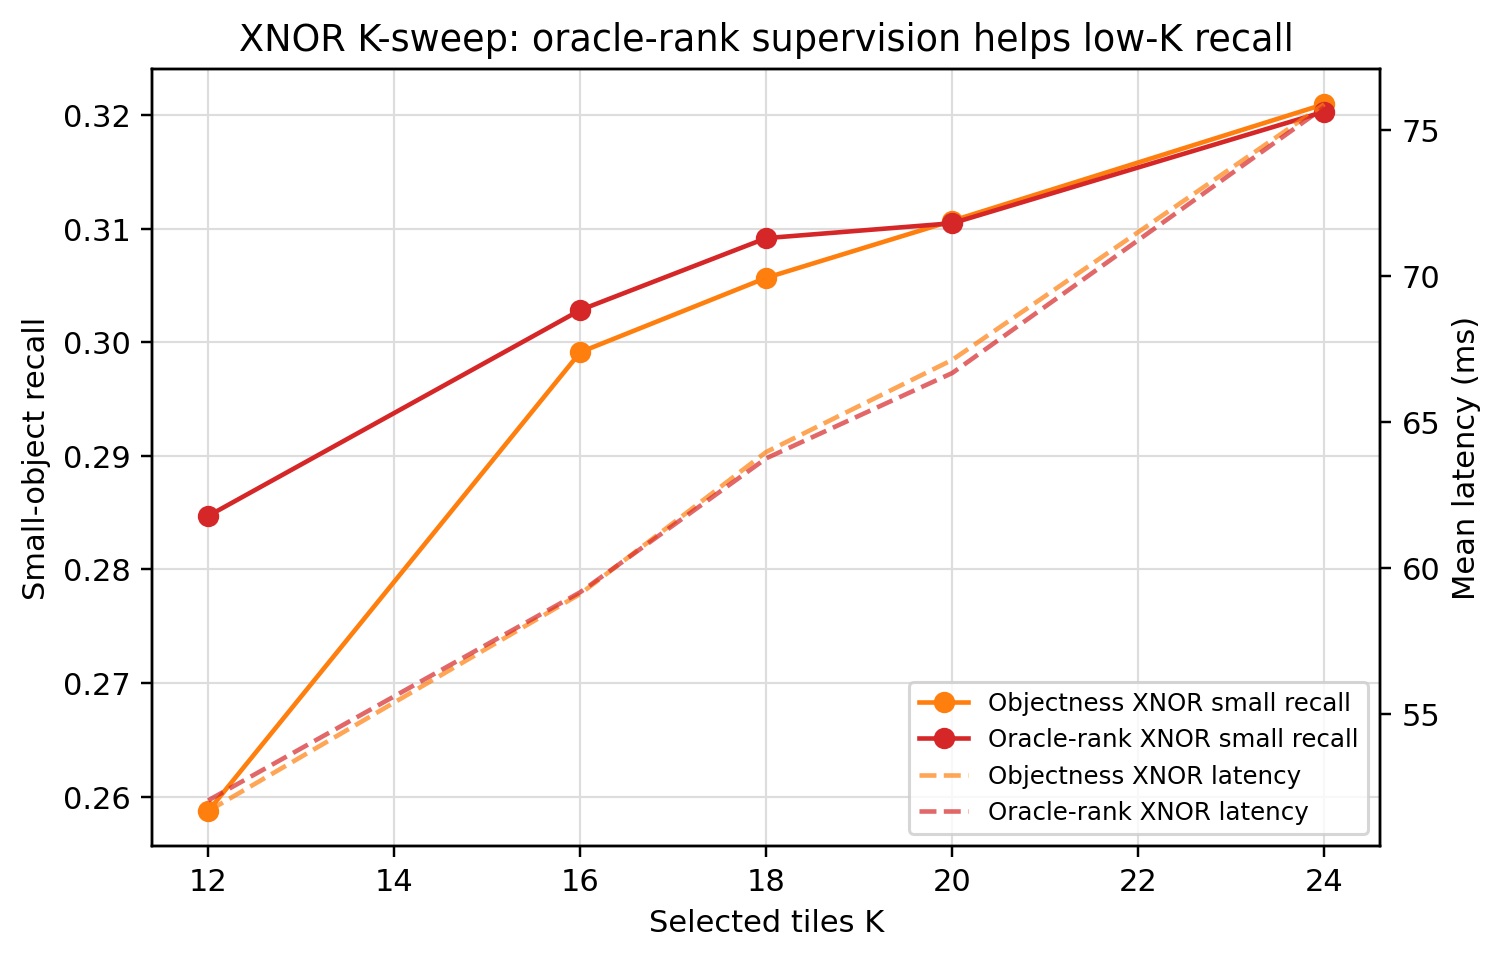
\includegraphics[width=\linewidth]{xnor_k_sweep.png}
\caption{Native XNOR K-sweep. Oracle-rank supervision moves useful tiles earlier, especially at K12, but latency grows with the number of YOLO crops.}
\label{fig:xnor_sweep}
\end{figure}

The scout-only gate in Table~\ref{tab:scout_gate} shows why the oracle-rank model was worth testing. It improves object-center coverage at K12, K16, and K18 before full detector benchmarking. The detector-level improvement is smaller because object-center coverage does not perfectly predict final YOLO matches after crop detection and merging.

\begin{table}[t]
\centering
\caption{Scout-only object-center recall for native XNOR scouts on the full validation split.}
\label{tab:scout_gate}
\begin{tabular}{lrrrrr}
\toprule
Scout & $K=12$ & $K=16$ & $K=18$ & $K=20$ & $K=24$ \\
\midrule
Objectness XNOR & 0.767 & 0.899 & 0.942 & 0.964 & 0.973 \\
Oracle-rank XNOR & 0.833 & 0.922 & 0.946 & 0.960 & 0.969 \\
\bottomrule
\end{tabular}
\end{table}

\section{Discussion}
The strongest positive result is that selective tiling is a real opportunity. Exhaustive tiling improves small-object recall by a large margin, and oracle selection proves that many of the 49 tiles are redundant. Oracle K12 reaches 0.329 small-object recall at 32.9 ms, close to exhaustive tiling's 0.355 small-object recall at 107.2 ms.

The implemented binary/XNOR scout is a partial success. It is real, measured, and aligned with the intended operation split: CPU native XNOR scout selection followed by GPU YOLO detection. However, it does not meet the strict K18 target. The best low-K oracle-rank XNOR result is K18 at 0.344 recall, 0.309 small recall, and 63.8 ms. K24 recovers more small-object recall, but it uses more detector crops and should not be the headline low-cost result.

This does not invalidate the project. It gives a useful negative/partial result: the bottleneck is no longer the tiling concept or YOLO integration, but fixed-K ranking quality and CPU/Python scout overhead. On a desktop RTX 4090, the learned GPU heatmap is a strong reference because it benefits from optimized GPU execution. The edge-device motivation remains plausible, but it was not proven without Jetson-class hardware measurements.

\section{Conclusion}
The project produced a runnable and benchmarked scout-guided tiling pipeline for UAV small-object detection. The evidence supports three final claims: full-image YOLO misses many small objects, exhaustive tiling recovers much of that recall at high cost, and selective tile routing is a promising way to trade recall against compute. The binary/XNOR scout partially validates the original idea but does not fully reach the proposed speed/recall target in the final benchmark.

Future work should focus on improving tile-ranking quality, reducing native scout overhead, benchmarking on actual edge hardware, and fine-tuning the detector on VisDrone if official mAP is required. The custom detector loss from the presentation should only be revisited after the routing experiment is stable, because it changes the project from routing efficiency to detector optimization.

\section*{Individual Contributions}
Replace this with the final agreed group contributions before submission:
\begin{itemize}
\item Student 1: dataset preparation, benchmark execution, report writing.
\item Student 2: native C/XNOR kernel, packed binary verification, Windows build support.
\item Student 3: scout/routing implementation, tile contracts, evaluation scripts.
\item Student 4: YOLO detector runner, result analysis, presentation/report figures.
\end{itemize}

\section*{Reproducibility Notes}
The main benchmark artifact is \texttt{artifacts/benchmarks/oracle\_rank\_final/summary.md}. The code includes correctness checks for the native packed kernel, tile contracts, routing, heatmap scout, XNOR heatmap scout, and detector utilities. The final report figures are generated from frozen JSON artifacts with \texttt{scripts/make\_final\_report\_figures.py}.

\bibliographystyle{IEEEtran}
\bibliography{references}

\end{document}
